\section{Установка и настройка комплекса}

\subsection{Подготовка серверной ОС}

Для установки используется бесплатная демо-версия, позволяющая использовать все функции
ОС в течение 180 дней. Для тестирования будет использована версия Standart, т.к.
версия Essentials активируется только после ввода лицензионного ключа. Процесс установки
показан на рисунках \ref{pic:install-1}–\ref{pic:install-4}.

\begin{figure}[p]
    \center
    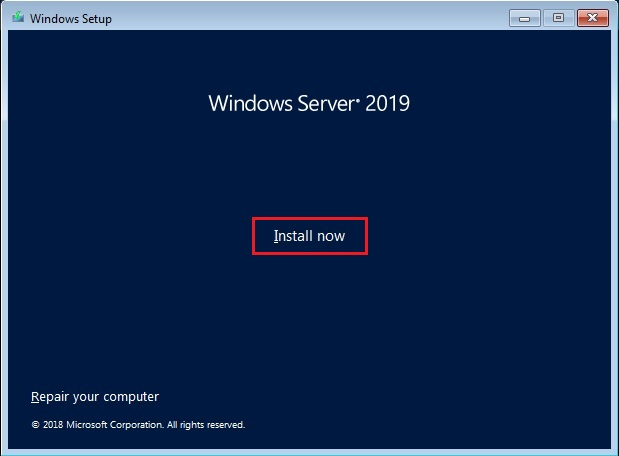
\includegraphics[height=10cm]{install-1}
    \caption{Главное окно установщика}
    \label{pic:install-1}
\end{figure}

\begin{figure}[p]
    \center
    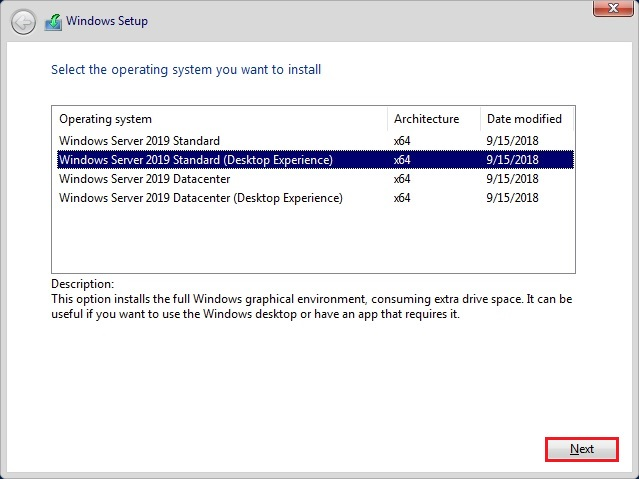
\includegraphics[height=10cm]{install-2}
    \caption{Выбор редакции}
    \label{pic:install-2}
\end{figure}

\begin{figure}[p]
    \center
    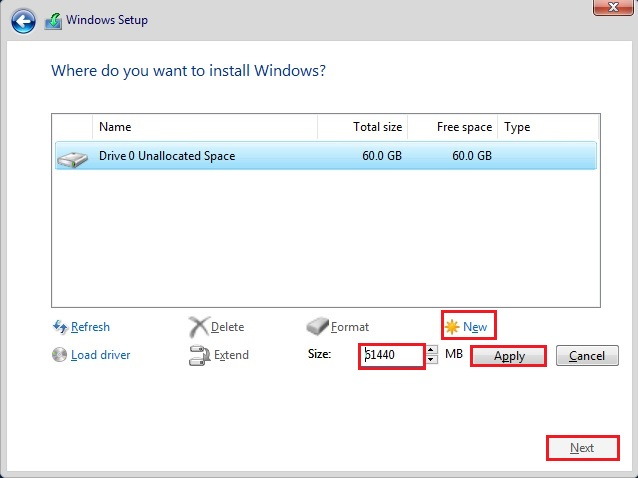
\includegraphics[height=10cm]{install-3}
    \caption{Выбор диска для установки}
    \label{pic:install-3}
\end{figure}

\begin{figure}[p]
    \center
    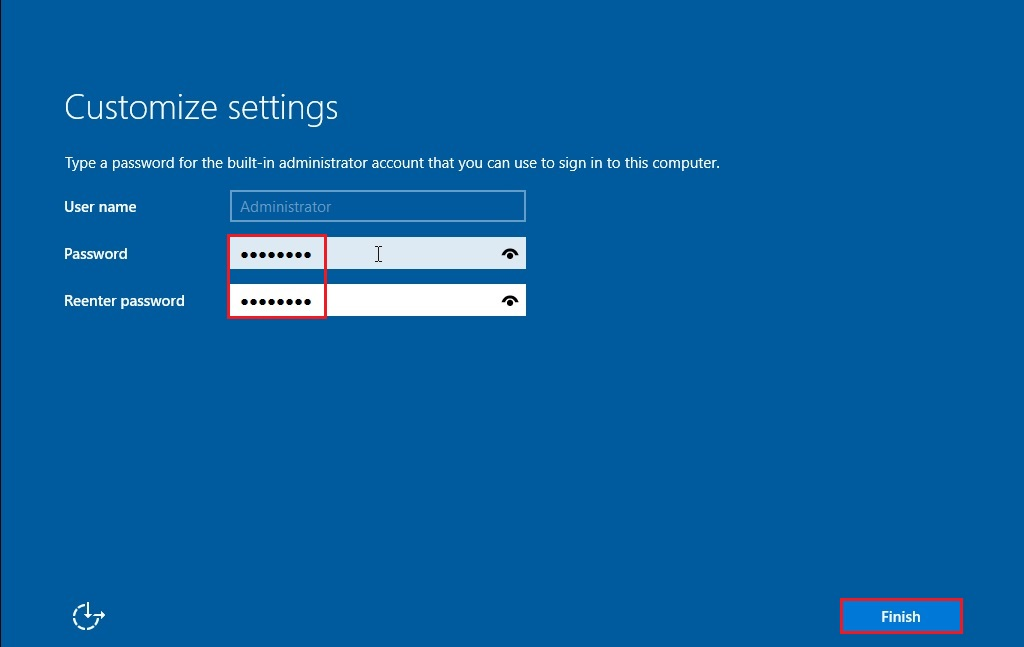
\includegraphics[height=10cm]{install-4}
    \caption{Создание учетной записи администратора}
    \label{pic:install-4}
\end{figure}

\begin{figure}[p]
    \center
    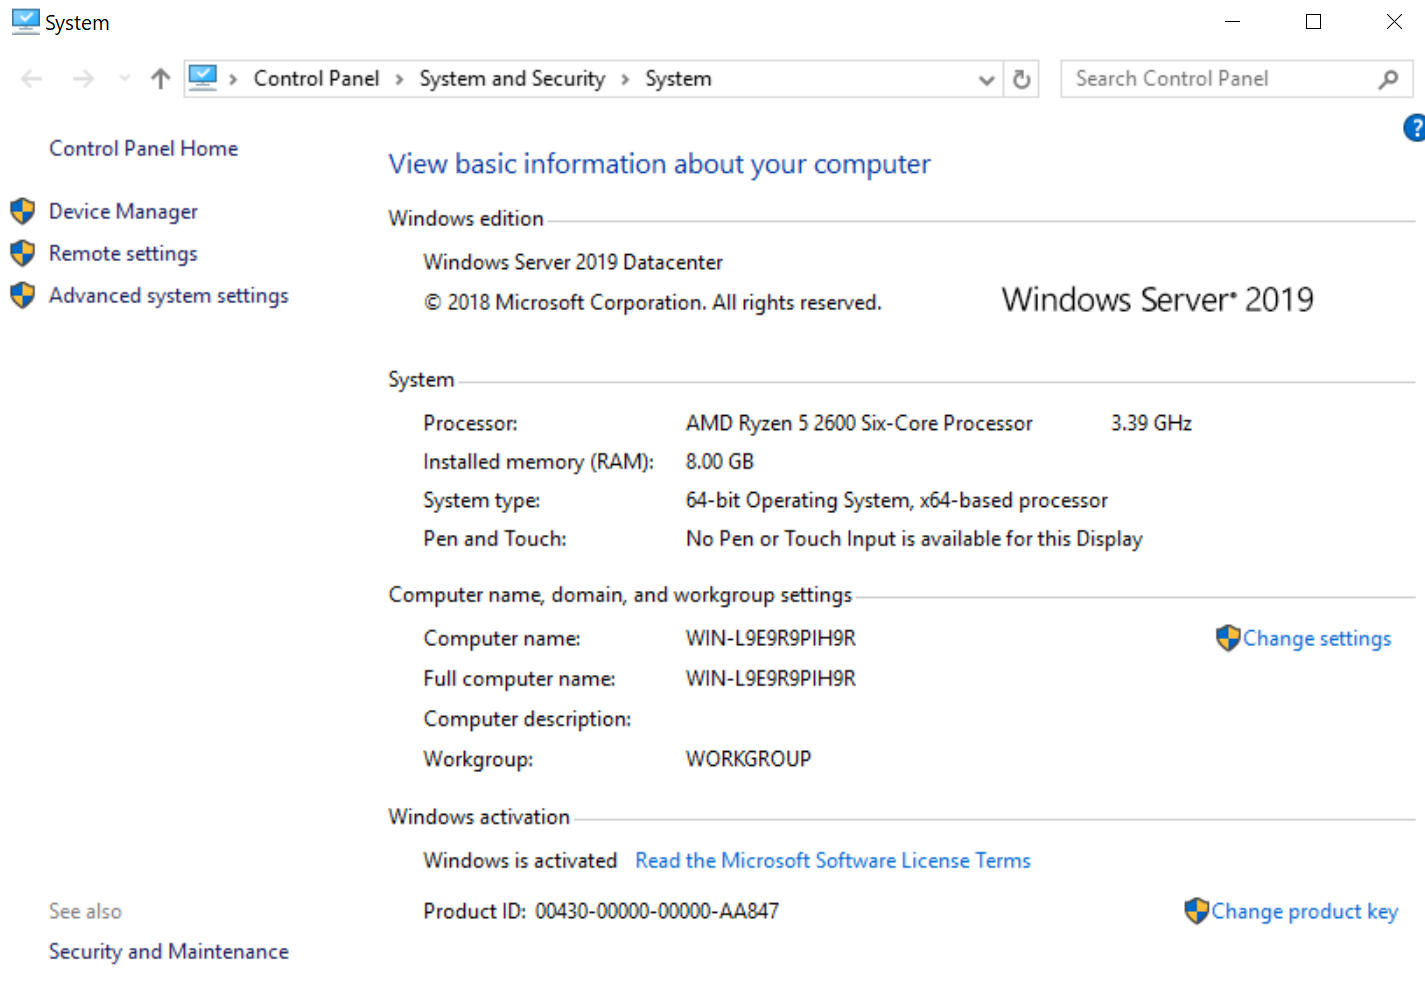
\includegraphics[height=10cm]{install-info}
    \caption{Сведения о установленной системе}
    \label{pic:install-info}
\end{figure}

\begin{figure}[p]
    \center
    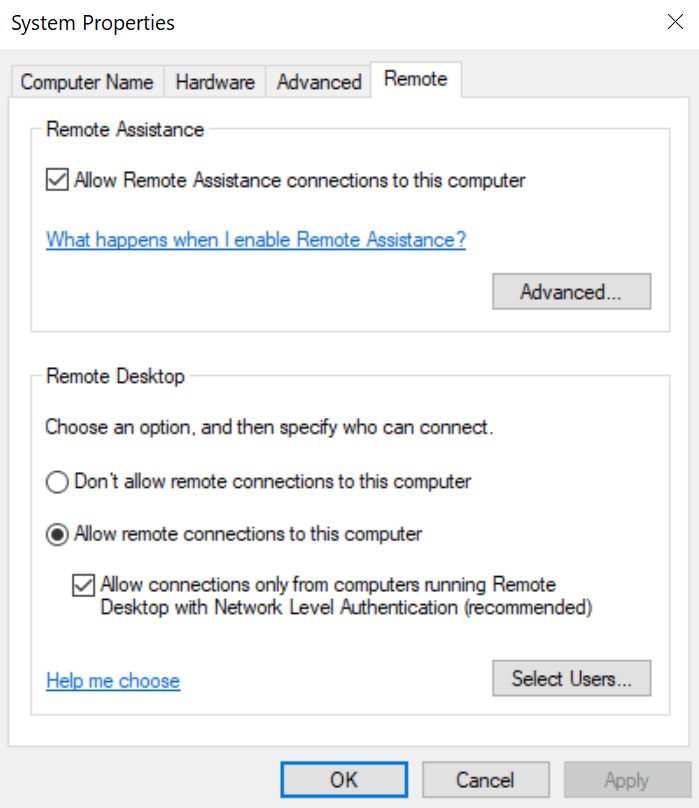
\includegraphics[height=10cm]{install-rdp}
    \caption{Включение доступа по RDP}
    \label{pic:install-rdp}
\end{figure}

\begin{figure}[h]
    \center
    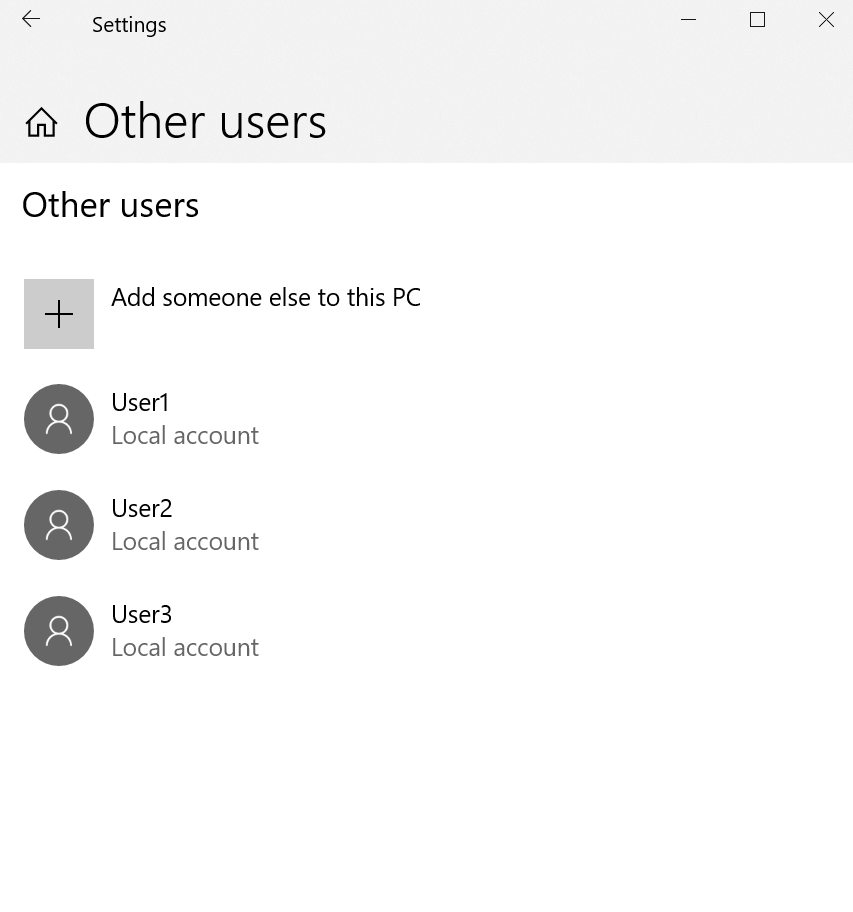
\includegraphics[height=10cm]{install-users}
    \caption{Добавление пользователей}
    \label{pic:install-users}
\end{figure}

В результате установки доступны все функции Windows Server (см.
рисунок~\ref{pic:install-info}). Нужно добавить возможность подключения по RDP
(см. рисунок~\ref{pic:install-rdp}). Также для работы нужно добавить в систему пользователей
для тонких клиентов. Добавлены пользователи \texttt{User1} – \texttt{User3} (см.
рисунок~\ref{pic:install-users}). Установка клиентского ПО (различные САПР, офисные
пакеты и т.д.) в работе не рассматривается.
